\documentclass[palatino]{epflnotes}

\title{Instability}
\author{Guillermo Julián Moreno}
\date{16/17 - Fall semester}

% Additional packages
\usepackage{tikztools}
\usepackage{caption}
% --------------------

\begin{document}
\frontmatter
\pagestyle{plain}
\maketitle

\tableofcontents
\mainmatter
% Content

\chapter{Introduction and basic definitions}

\section{Stability}

\begin{defn}[Monotonous stability][Stability!monotonous] A system where, given an initial disturbance of the energy $E$, it tends to the stable state with monotonically decreasing energy function.
\end{defn}

\begin{defn}[Asymptotic stability][Stability!asymptotic] A system where, given an initial energy disturbance, it tends to the stable state with no restrictions on the shape of the function.
\end{defn}

\begin{defn}[Conditional stability][Stability!conditional] A system where the stable state depends of the quantity of the initial disturbance.
\end{defn}

\begin{defn}[Inconditional instability][Instability!inconditional] I don't think this deserves a definition. In some instances we will be interested in small increments of time in order to be able to linearize the equation.
\end{defn}

\section{Case study: dynamical system of a rotating ring}

\begin{figure}[hbtp]
\centering
\inputtikz{RotatingRing}
\caption{A ball in a rotating ring has two different forces: centrifugal and gravity. When the projection of these two are equal, the ball will not move and will thus reach an equilibrum (stable state).}
\label{fig:Introduction:RotatingRing}
\end{figure}

We will study an example of conditional stability: a ball of mass $m$ in a ring of radius $R$ as in \fref{fig:Introduction:RotatingRing}. We want to find the stable state, in which the projections of the centrifugal and gravity forces over the tangent line to the ring cancel themselves.

The gravity force is easy enough: $-mg$ being $g$ the acceleration of gravity. Centrifugal force is easy too: we only have to take into account that the radius at which the ball is rotating (dotted orange path on the figure) depends on the angle θ, simply by $r = R \sin θ$. Thus, the centrifugal force is $mRω^2\cos ω $.

Adding these two forces projected accordingly over the tangent line to the circle (purple line i \fref{fig:Introduction:RotatingRing}) we have the resultant force $F$ exerted over the ball: \( F = -mg\sin θ + mRω^2 \sin θ \cos θ\)

We can substitute the force by the expression $mR\ddot{θ}$ where $\ddot{θ}$ is the angular acceleration of the ball. This gives us the final differential equation for the ball in a rotating ring movement: \( mR\ddot{θ} = -m g \sin θ + m R ω^2 \sin θ \cos θ \label{eq:Introduction:RotatingRingEquationComplete} \)

We can simplify this equation by defining $ω_0^2 = \frac{g}{R}$ as the pendulum frequency, which we will see later why it is interesting. A straightforward substitution yields a simpler equation: \( \ddot{θ} = -ω_0^2 \sin θ + ω^2 \sin θ \cos θ \label{eq:Introduction:RotatingRingEquation} \)

This is not a differential equation that can be solved in a straightforward way. However, we can study what happens when we add a small perturbation.

Our base, stable case is $θ = 0$, which is obviously a solution of \eqref{eq:Introduction:RotatingRingEquation}. What happens when we start with $θ(0) = ε$, with $ε > 0$ as small as required?

Given that ε is small, we can approximate $\sin ε \approx ε$ and $\cos ε \approx 1$ so that our equation becomes \( \ddot{θ} = -ω_0^2 θ + ω^2 θ = (ω^2 - ω_0^2) θ \label{eq:Introduction:RotatingRingSimple} \)

The solution to this simplified differential equation is \( θ = c_1 e^{\sqrt{ω^2 - ω_0^2} t} + c_2 e^{-\sqrt{ω^2 - ω_0^2} t} \label{eq:Introduction:PendulumSolution} \) with $c_1, c_2$ constants depending on the initial conditions. Let's calculate them, as we will need them later to describe the equations. For simplicity, we can suppose that the initial velocity is null ($\dot{θ}(0) = 0$) and thus what we end up with is that $c_1 = c_2 = \sfrac{ε}{2}$

Now on to the actual interesting part: study the behaviour of the solution depending on the value of $ω^2 - ω_0^2$. If $ω^2 < ω_0^2$, the square root is imaginary and our solution will be a cosine: $θ(t) = ε \cos \left[(ω_0^2 - ω^2) t\right]$\footnote{Notice the sign change on $ω_0^2 - ω^2$, important because we want to get the imaginary value out of the square root.}. Thus, in this case the ball will only oscillate between the angles $θ = \pm ε$.

However, if $ω^2 > ω_0^2$, things change. In this case the square root is real, and thus the solution grows exponentially to infinity (first exponential grows, second one quickly decreases to 0 as it has a negative sign). This would be the \textbf{unstable} situation.

An interesting phenomenon is that when we are in the stable zone ($ω^2 < ω_0^2$) but with both quantities very similar, the relaxation time (that is, the time it takes to the system to go back to the stable state) starts to grow up to infinity.

\subsection{Equilibrum states}

\begin{figure}[hbtp]
\inputtikz{RotatingRingStableSolutions}
\caption{Equilibrum points of the rotating ring system with arrows describing whether it's a stable (attracting) or unstable state. The solution $θ_0$ becomes unstable with $\sfrac{ω^2}{ω_0^2} > 1$.}
\label{fig:Introduction:RotatingRingStable}
\end{figure}

Equilibrum states are those that arise as constant functions. Solving \eqref{eq:Introduction:RotatingRingEquation} for $θ = c$ constant, we get first $θ_0 = 0$ and \[ θ_s = \pm \arccos\left(\frac{ω_0^2}{ω^2}\right)\] as solutions, where the latter is only defined for $ω^2 ≥ ω_0^2$. This leads to a bifurcation, as can be seen on \fref{fig:Introduction:RotatingRingStable}.

In order to see that these states are actually stable and not static but unstable points is to see what happens with small perturbations. Thus, we would study the case with initial flow $θ(0) = θ_s \pm εθ'$, and then see what does the solution tend to. I would do it but I don't want to deal with nasty trigonometric calculations, that's for engineers.

After those nasty computations, we would end up with a simplified equation for $θ'$ given by \[ \ddot{θ}' = -θ'ω^2 \sin^2 θ_s \] whose solution is a pure imaginary exponential. That is, we have an stable value.

\chapter{Instabilities}

\section{Rayleigh-Taylor instability}

\begin{figure}[hbtp]
\begin{minipage}[b]{0.45\textwidth}
\centering
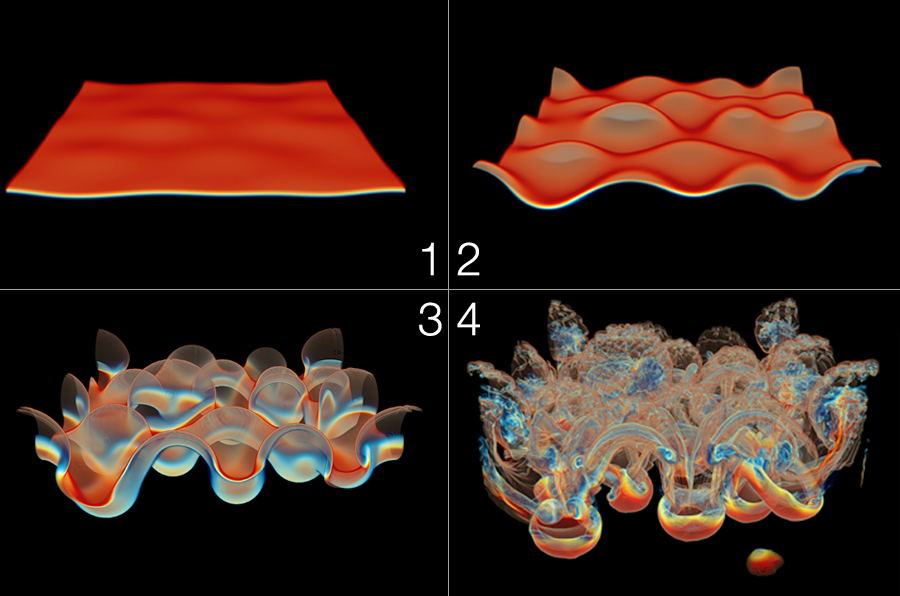
\includegraphics[width=0.8\textwidth]{img/RayleighTaylorInstability.png}
\captionof{figure}{Image of the evolution of the interface with Rayleigh-Taylor instability.}
\label{fig:RayleighTaylorInterfaceImage}
\end{minipage}
\hfill
\begin{minipage}[b]{0.45\textwidth}
\inputtikz{RayleighTaylorModel}
\captionof{figure}{Simplified model of two liquids: 2D and with infinite semiplanes.}
\label{fig:RayleighTaylorModel}
\end{minipage}
\end{figure}

Our first instability will be Rayleigh-Taylor, which models a situation with two impermeable liquids, one below of the other.

To simplify the study of these kind of instabilities, we simplify down to a situation like in \fref{fig:RayleighTaylorModel}. We assume a potential flow with no rotation and no vorticity. Then, to study it we will follow the steps outlined previously.

Our potential flow is $ΔΦ_1 = ΔΦ_2 = 0$, so our velocity equations are \begin{align*}
U_1 &= \dpd{Φ_1}{x} & V_1 = \dpd{Φ_1}{z} \\
U_2 &= \dpd{Φ_2}{x} & V_2 = \dpd{Φ_2}{z}
\end{align*}

The velocities $U$ represent the movement of the flow parallel to the $x$ axis, and $V$ represents the velocity parallel to the $z$ axis.

The boundary conditions will be zero values for $Φ_1$ and $Φ_2$ at $z = \pm ∞$ respectively: we don't want the flows to move at infinity.

The next step is the definition of the interface, the set of points where the two flows ``touch'', and define the relations at that boundary. The first one is impermeability: no particles pass through the interface. This means that, as reflected in \fref{fig:RayleighTaylorInterface}, the components of $V_1$ and $U_1$ normal to the interface ($V_\perp$ and $U_\perp$) must cancel. Knowing also that, at the interface, $V_1 = ∂_t η$, we can start writing down the expressions of that:
\begin{align*}
V_\perp &= ∂_t η \cos α \\
U_\perp &= U_1 \sin α
\end{align*}

\begin{figure}
\inputtikz{RayleighTaylorInterface}
\caption{Interface η in Rayleigh-Taylor instability.}
\label{fig:RayleighTaylorInterface}
\end{figure}

Our kinematic condition is that we will force impermeability, so that normal components to the interface must be equal. Now for the fluid we write down some equations and something.

Now on to the dynamic boundary conditions.

For potential flows, we have the second Bernouilli relations:
\begin{align*}
\dpd{Φ_1}{t} + \frac{U_1^2 + V_1^2}{2} + \frac{P_1}{ρ_1} + gz &= C_1(t) \\
\dpd{Φ_2}{t} + \frac{U_2^2 + V_2^2}{2} + \frac{P_2}{ρ_2} + gz &= C_2(t) \\
\end{align*}

Looking at these relations at infinity, we assume that nothing changes there so we can equate $C_1(t) = C_2(t) = 0$ and life is easier.

Once we have this, we add a small perturbation $ε$ to everything.

Then a lot of linearization without checking if the functions involved are analytic.

Then double Fourier analysis (normal mode expansion). Mumbojumbo. Solutions. Eigenvalue and a dispersion relation for a non-trivial solution.

\appendix

% \chapter{---}
% % -*- root: ../Instability.tex -*-
\section{Instability of a thin suspended film}

Something something.

\backmatter
\printindex
\end{document}
